\documentclass[specialist, 12pt, href]{article}
\usepackage[utf8]{inputenc}
\usepackage[russian]{babel}
\usepackage[T2A]{fontenc}
\usepackage{indentfirst}
\usepackage{caption}
\usepackage{latexsym,amssymb,amsthm}
\usepackage{amsfonts}
\usepackage{amsmath}
\usepackage{graphicx}
\usepackage{subfigure}

\usepackage[a4paper, includefoot,
            left=2cm, right=2cm,
            top=2cm, bottom=2cm,
            headsep=1cm, footskip=1cm]{geometry}

\usepackage{hyperref}
\setcounter{tocdepth}{2}
\allowdisplaybreaks[4]

\linespread{1.2}
\title{Boosting}
\author{Зиннатулина Белла}
\date{}

\begin{document}
\maketitle



\section{Введение}

В сфере анализа данных существует множество методов решения уже классических задач регрессии и классификации.  
При построении прогноза возникает задача минимизации эмпирического риска. В данном конспекте рассматривается идея построения композиции алгоритмов. 

\section{Постановка задачи}

Рассматривается задача обучения $<X,Y, f, X^{n}>$, где  \begin{itemize}
 \item $X$ --- пространство объектов, $Y$ --- можество ответов,
 \item $f: X \mapsto Y$ --- неизвестная целевая зависимость,
 \item $X^{n} = (x_1,\dots,x_{n})$ --- обучающая выборка,
 \item $Y^{n} = (y_1,\dots, y_{n})$ --- вектор ответов на обучающих объектах, где $y_i = f(x_i)$,
 \item $a(x) = C(b(x))$ --- алгоритм, аппроксимирующий целевую зависимость $f$ на всем множестве $X$,
 \item $b:X \mapsto R$ --- базовый алгоритм,
 \item $C:R \mapsto Y$ --- решающее правило,
 \item $R$ --- пространство оценок.
 \end{itemize}

В случае решения задачи классификации значением $b(x)$ может являться вероятность принадлежности объекта $x$ классу, которое решающее правило $C$ переводит в номер класса. В случае же регрессии $C(b) \equiv b$.

Boosting основывается на двух идеях: изменении постановки задачи таким образом, что вместо одного базового алгоритма $b$ рассматривается несколько, и в жадной стратегии решения такой задачи.

\subsection*{Первая идея: изменение постановки задачи}
 
Мы будем рассматривать (параметризованное) множество базовых алгоритмов $\mathcal{B} = \mathcal B(\Theta) = \{b(\cdot; \theta) | \theta \in \Theta\}$.
В дальнейшем, говоря о “выборе очередного базового алгоритма”, мы будем, для краткости, писать $b(x)$, подразумевая, что на самом деле выбирается некое $\theta \in \Theta$ и $b(x) = b(x; \theta) \in \mathcal B(\Theta)$.

\textbf{Определение.} Композиция базовых алгоритмов $b_1,\dots, b_T \in \mathcal{B}$ имеет вид
$$a(x) = C(F(b_1(x),\ldots,b_T(x); \omega)),$$ 
где $F:R^T \mapsto R$ называют \textit{корректирующей} операцией, параметризованной с помощью $\omega \in \Omega$.

Смысл этого определения заключается в том, что вместо одного алгоритма $b$ рассматривается сразу $T$ базовых алгоритмов $b_1(x)$, $b_2(x)$, \ldots $b_T(x)$, а $F$ <<агрегирует>> значения базовых алгоритмов.

Например, $F$ может быть линейной функцией, то есть 
$\omega= (\omega_1, \ldots, \omega_T) \in \mathbb R^T$ и 
$$ F(b_1(x),\ldots,b_T(x); \omega) = \sum_{t=1}^T \omega_t b_t(x). $$
В дальнейшем, мы всегда будем считать  $F$ линейной в указанном выше смысле
и писать $F(b_1(x),\ldots,b_T(x))$ вместо $F(b_1(x),\ldots,b_T(x); \omega)$.

В таких обозначениях задача формулируется, как подбор оптимальных (в смысле рассматриваемой функции потерь) параметров $\omega$ и базовых алгоритмов $\{b_t(x)\}_{t=1}^T$.

\subsection*{Вторая идея: жадность алгоритма}
Как всегда, начинать нужно с попытки точно решить задачу.
Заметим, однако, что оптимизация функции потерь происходит по многомерному множеству параметров.
В связи с этим точная многомерная оптимизация не выглядит перспективной.

Концептуальная идея Boosting заключается в использовании \textbf{жадной} стратегии оптимизации.
Неформально идею можно следующим образом.
Пусть для некоторого фиксированного $T_0 < T$ мы (уже) выбрали алгоритмы $\{b_t\}_{t=1}^{T_0}$ и параметры корректирующей функции $\{\omega_t\}_{t=1}^{T_0}$.
На $(T_0 + 1)$-ом шаге <<жадной>> процедуры мы выбираем параметр $\omega_{T_0+1}$ и базовый алгоритм $b_{T_0 + 1}$ из тех соображений, чтобы исправить “ошибки”, допущенные композицией, основанной лишь на первых  $T_0$ алгоритмах.
Иными словами выбор очередного параметра и базового алгоритма происходит для исправления ошибок
$$ a(x) = C\left(\sum_{t=1}^{T_0} \omega_t b_t(x)\right). $$
При этом алгоритмы $\{b_t\}_{t=1}^{T_0}$ и параметры корректирующей функции $\{\omega_t\}_{t=1}^{T_0}$ остаются без изменений.
 

Для того, чтобы прояснить эту абстрактную концепцию обратимся к следующему примеру.

\textbf{Пример 1.} Рассмотрим задачу регрессии. В этом случае $C(b) = b, Y = \mathbb{R}, R = \mathbb{R}$ (по существу, решающее правило отсутствует).

Пусть $F(b_1(x),\ldots,b_T(x)) = \sum\limits_{t = 1}^{T}{b_t(x)}, x \in X$.

Обучим простой алгоритм $b_1(x) = \underset{b \in \mathcal{B}}{\arg\min} \frac{1}{n}\sum\limits_{i = 1}^{n}{(b(x_i) - y_i)^2}$. Добавим алгоритм $b_2$, исправляющий ошибки $b_1$: $b_1(x_i) + b_2(x_i) = y_i$.

Получили поправку $y_i-b_1(x_i) \mapsto$ $b_2(x) =  \underset{b  \in \mathcal{B}}{\arg\min} \frac{1}{n}\sum\limits_{i = 1}^{n}{(b(x_i) -(b_1(x_i) - y_i))^2} \mapsto$

$b_T(x) =  \underset{b  \in \mathcal{B}}{\arg\min} \frac{1}{n}\sum\limits_{i = 1}^{n}{(b(x_i) -(\sum\limits_{t = 1}^{T-1}b_t(x_i) - y_i))^2}$.

Заметим, что вместо
$$F(b_1(x),\ldots,b_T(x)) = \sum\limits_{t = 1}^{T}{b_t(x)}, x \in X,$$
можно рассмотреть
$$F(b_1(x),\ldots,b_T(x)) = \frac{1}{n} \sum\limits_{t = 1}^{T}{b_t(x)}, x \in X.$$
Однако, в такой ситуации есть намек на <<равноправность>> базовых алгоритмов между собой, будто бы между ними происходит <<голосование>>.
В действительности, очередной алгоритм пытается исправлять ошибки предыдущих.

\section{AdaBoost}

Рассмотрим задачу классификации на два класса.
$Y = \{-1,1\}$ и определим решающее правило $C(b) = sign(b)$.
Тогда $b_t:X \mapsto \{-1,0,1\}, b_t \in \mathcal{B}$.
Случай, когда $b_t(x) = 0$, следует понимать как отказ базового алгоритма $b_t$ от классификации объекта $x$.

Положим $F(b_1(x),\dots,b_t(x)) = \sum\limits_{t = 1}^{T}{\omega_tb_t(x)} \mapsto a(x) = sign(\sum\limits_{t = 1}^{T}{\omega_tb_t(x)}), x \in X$.

Функционал качества композиции определяется как число ошибок, допускаемых на обучающей выборке: $Q_T = \sum\limits_{i=1}^n{[y_i\sum\limits_{t=1}^T\omega_tb_t(x_i) \leq 0]}$.

Конечно, прямая оптимизация такого функционала является затруднительной.
Поэтому $Q_T$ мажорируется некоторой непрерывно дифференцируемой функцией, поддающейся эффективной оптимизации.

На Рис.\ref{fig:approx} представлены различные варианты гладких мажорант.

Выбор функции для аппроксимации зависит от характера задачи.
Например, логарифмическая функция связана с принципом максимума правдоподобия и применяется в логистической регрессии, кусочно-линейная аппроксимация связана с принципом максимизации зазора между классами.


\begin{figure}[h!]
\centering
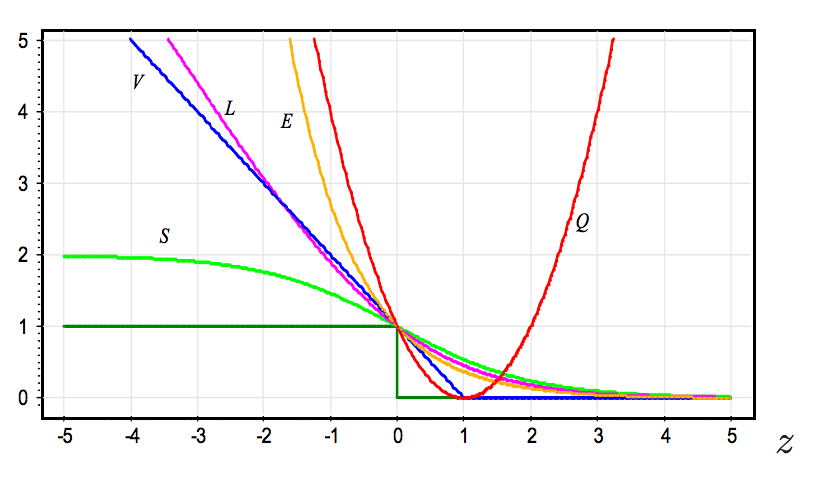
\includegraphics[width = 5in]{fig/approx.png}
\captionsetup{singlelinecheck=off}
\caption[]{Гладкие верхние аппроксимации пороговой функции потерь $[z < 0]$:
\begin{itemize}
 \item[] $S(z) = 2(1 + \exp(z))^{-1}$ --- сигмоидная;
 \item[] $L(z) = \log_{2} (1 + \exp(-z))$ --- логарифмическая;
 \item[] $V(z) = (1 - z)_+$ --- кусочно-линейная;
 \item[] $E(z) = \exp(-z)$ --- экспоненциальная;
 \item[] $Q(z) = (1 - z)^2$ --- квадратичная.
\end{itemize}}
\label{fig:approx}
\end{figure}
\newpage
Алгоритм AdaBoost использует экспоненциальную аппроксимацию.
Оценка функционала $Q_T$ сверху имеет вид:
$$ Q_T \leq \tilde Q_T = \sum \limits _{i = 1} ^ n \underset{v_i}{\underbrace{exp\{-y_i\sum\limits_{t=1}^{T-1}\omega_tb_t(x_i)}\}} exp\{-y_i\omega_Tb_T(x_i)\}.$$

Введём вектор нормированных весов объектов $\tilde  V_n = (\tilde v_1,\dots,\tilde v_n), \tilde  v_i =  v_i / \sum \limits _{j = 1}^n v_j$.

Далее определим два функционала качества алгоритма классификации $b$ на обучающей выборке $X^n, Y^n$
с нормированным вектором весов объектов $U_n = (u_1 \dots,u_n)$ --- суммарный вес ошибочных (negative)  классификаций $N(b;U_n)$ и суммарный вес верных (positive) классификаций $P(b; U_n)$:

$N(b, U_n) = \sum\limits_{i = 1}^n  u_i[b(x_i) = -y_i], \quad P(b, U_n) = \sum\limits_{i = 1}^n  u_i[b(x_i) = y_i].$

Стоит отметить, что при отсутствии отказов алгоритма от классификации, $N + P = 1$.

\textbf{Теорема 1(Freund, Schapire, 1996).} Пусть для любого нормированного вектора весов $ U_n$ существует алгоритм $b \in \mathcal{B}$: $P(b, U_n) > N(b, U_n)$. \\
Тогда минимум функционала $\tilde Q_T$ достигается при
$b_T =  \underset{b  \in \mathcal{B}}{\arg\max} \sqrt{P(b;\tilde V_n)} - \sqrt{N(b;\tilde V_n)}$, $\omega_T = \frac{1}{2} \ln\frac{P(b_T,\tilde V_n)}{N(b_T,\tilde V_n)}$.

Иными словами требуется существование алгоритма $b \in \mathcal{B}$, который классифицирует выборку <<чуть лучше, чем наугад>>.


Пусть $b_t: X \mapsto \{-1;+1\}$. Тогда $P = 1 - N$.

\textbf{Теорема 2(Freund, Schapire, 1995).} Пусть для любого нормированного вектора весов $ U_n$ существует алгоритм $b \in \mathcal{B}$: $N(b, U_n) < \frac{1}{2}$.
Тогда минимум функционала $\tilde Q_T$ достигается при 
$b_T =  \underset{b  \in \mathcal{B}}{\arg\min} N(b;\tilde V_n)$, $\omega_T = \frac{1}{2} \ln\frac{1 - N(b_T,\tilde V_n)}{N(b_T,\tilde V_n)}$.

\subsection*{Алгоритм AdaBoost}

{\bf {Вход}}: $X^n, T$.

{\bf {Выход}}: $\omega_t, b_t, t = 1,\dots,T$.
\begin{enumerate}
   \item $v_i := 1/n, i = 1,\dots,n$;
   \item для всех $t = 1,\dots,T$
   \item \quad обучить базовый алгоритм: $b_T =  \underset{b  \in \mathcal{B}}{\arg\min} N(b;V_n)$;
   \item \quad $\omega_T = \frac{1}{2} \ln\frac{1 - N(b_T,\tilde V_n)}{N(b_T, V_n)}$;
   \item \quad пересчитать веса объектов: $u_i := u_i \exp\{-\omega_t y_i b_t(x_i)\}, i = 1,\dots,n$;
   \item \quad нормировать веса объектов: $v_0 := \sum\limits_{j=1}^n v_i$; $v_i := v_i/v_0, i = 1,\dots,n$;
\end{enumerate}

\section{Градиентный бустинг}

Исторически сложилось, что первым появился алгоритм AdaBoost, который использует экспоненциальную аппроксимацию. 
Теперь же рассмотрим общий случай, когда пороговая функция потерь $Q_T$ оценивается сверху произвольной невозрастающей функцией $\mathcal{L}(a,y),$ где 
$$a(x) = \sum\limits_{t=1}^T \omega_t b_t(x), \quad x \in X, \quad \omega_t \in \mathbb{R}_+.$$

Функционал качества имеет вид:
$$Q_T \leq \tilde Q_T= \sum \limits_{i = 1}^n \mathcal{L} \underbrace{\bigg ( \underset{f_{T-1,i}}{\underbrace{y_i\sum\limits_{t=1}^{T-1} \omega_t b_t(x_i)}} + y_i\omega_T b_T(x_i) }_{f_{T, i}}\bigg),$$

где $ \mathcal{L}(a,y)$ --- произвольная функция потерь,
 
$f_{T-1} = (f_{T-1,i})_{i=1}^n $ --- текущее приближение 

$f_T = (f_{T,i})_{i=1}^n $ --- следующее приближение.

Рассмотрим функцию потерь $\mathcal{L}$ как функцию от параметра $\omega_T$:

$$\lambda(\omega_T) := \mathcal{L}(f_{T-1,i} + y_i\omega_T b_T(x_i)).$$

Линеаризуем $\lambda(\omega_T)$ в окрестности $\omega_T = 0$, разложив в ряд Тейлора и отбросив старшие члены:

$$\lambda(\omega_T) \approx \lambda(0) + \omega_T \lambda^ \prime (0)^,$$ 

что приведет к линеаризации функционала $\tilde Q_T$ по параметру $omega_T$:

$$\tilde Q_T \approx \sum \limits_{i = 1}^n \mathcal{L}(f_{T-1,i}) - \omega_T \sum \limits_{i = 1}^n\underset{v_i}{\underbrace{ -\mathcal{L} ^ \prime (f_{T-1,i})}} y_ib_T(x_i),$$

где $v_i$ --- веса объектов.

Для минимизации функционала качества $\tilde Q_T$ будем искать такой базовый алгоритм $b_T$, что $\{b_T(x_i)\}_{i = 1}^n$ приближает вектор антиградиента $\{-\mathcal{L} ^ \prime (f_{T-1,i})\}_{i = 1}^n:$

$$b_T := \underset{b  \in \mathcal{B}}{\arg\max} \sum\limits_{i=1}^n \bigg(b(x_i) + \mathcal{L} ^ \prime (f_{T-1,i})\bigg)^2.$$
 
После построения $b_T$, параметр $\omega_T$ определяется путем одномерной минимизации функционала $\tilde Q_T$.
Итерации этих двух шагов приводят к обобщённому
алгоритму бустинга AnyBoost.

\subsection*{Алгоритм AnyBoost}

{\bf {Вход}}: $X^n, Y^n$ --- обучающая выборка,

       \quad \qquad $T$ --- максимальное число базовых алгоритмов;.

{\bf {Выход}}: базовые алгоритмы и их веса $\omega_t, b_t, t = 1,\dots,T$.

\begin{enumerate}
    \item $f_i := 0, i = 1,\dots,n$;
    \item  Для всех $t = 1, \ldots,T$
    \item \quad найти базовый алгоритм, приближающий градиент:
    \item[] \quad$b_t:= \underset{b  \in \mathcal{B}}{\arg\max} \sum\limits_{i=1}^n (b(x_i) + \mathcal{L} ^ \prime (f_{i}))^2$;
    \item \quad$\omega_t := \underset{\omega > 0}{\arg\min} \sum\limits_{i=1}^n (\mathcal{L}(f_i + y_i\omega b_t(x_i)))^2$;
    \item \quad обновить значения $f_i$ на объектах выборки:
    \item[] \quad$f_i := f_i + \omega_t b_t(x_i), i = 1,\dots,n.$
 
\end{enumerate}

\section{ Заключение}

За всеми вышеописанными преимуществами бустинга стоит понимать, что метод не является уникальным решением любых, поставленных перед ним задач. 

\subsubsection*{Достоинства}
 \begin{itemize}
  \item Распределение весов объектов позволяет оценить наличие \textbf{выбросов}. Объекты с наибольшими весами $u_i$, скорее всего, являются выбросами.
  
  \item Бустинг является гибким алгоритмом, т.е. позволяет строить различные модификации.
  
  \item Прост в реализации.
  
  \item Временная сложность построения композиции практически полностью определяется временем обучения базовых алгоритмов.
  
 \end{itemize}



\subsubsection*{Недостатки}
 \begin{itemize}

 \item При наличии шума в данных AdaBoost может переобучиться. Экспоненциальная функция потерь слишком сильно увеличивает веса наиболее <<труднораспознаваемых>> объектов, на которых ошибаются многие базовые алгоритмы. Однако именно эти объекты чаще всего оказываются шумовыми выбросами. В результате AdaBoost начинает настраиваться на шум, что ведёт
к переобучению. 

  \item Жадная стратегия последовательного добавления базовых алгоритмов приводит к построению
неоптимального набора базовых алгоритмов. Для улучшения композиции можно периодически возвращаться к ранее построенным алгоритмам и обучать их
заново.

 \item AdaBoost требует достаточно длинных обучающих выборок, порядка $10^4 \ldots 10^6.$
 
 \item Бустинг может приводить к построению композиций, состоящих из сотен алгоритмов. Такие композиции решают поставленную задачу, к примеру, классификации, но исключают возможность содержательной интерпретации. В том числе требуют больших ресурсов памяти для хранения базовых алгоритмов и существенных затрат времени на вычисление классификаций.
  
 \end{itemize}

\subsubsection*{Существуют следующие рекомендации:}

\begin{itemize}

  \item На практике в качестве базовых классификаторов чаще всего используются деревья принятия решений. 
  
  \item В случае наличия объектов с большими весами $u_i$, стоит уделить им особое внимание, возможно, они являются выбросами, и их стоит исключить из рассмотрения и построить композицию заново.
  
 \end{itemize}

\end{document}
